\documentclass[report,11pt]{elsarticle}
%\documentclass{article}[11pt,a4]
%\documentclass[11pt]{article}

\usepackage[lined,linesnumbered]{algorithm2e}
\usepackage{a4wide}
\usepackage{ae}
\usepackage[czech,english]{babel}
\usepackage[utf8x]{inputenc}
\usepackage[T1]{fontenc}
\usepackage{graphicx}
\usepackage{url}
\usepackage{pdfpages}

\usepackage{listings}

\paperwidth=210 true mm
\paperheight=297 true mm
\pdfpagewidth=210 true mm
\pdfpageheight=297 true mm

% Pro cestinu zakomentuj nasledujici radek
%\selectlanguage{english}
% Pro anglictinu zakomentuj nasledujici radek
\selectlanguage{czech}

% Znakem procenta zacina komentovan

%%%% Pokud chcete
%%% odkomentu
%\usepackage[lined,linesnumbered]{algorithm2e}
%\usepackage{algorithm2e}
% Tento b
%\usepackage{ctable}
%\DeclareGraphicsExtensions{.pdf}

\begin{document}

\begin{frontmatter}

\title{Softwarový Projekt\\ Jazyk pro definici uživatelského rozhraní}

\author{Michal Hotovec\footnote{A4M39SVP -- Michal Hotovec, zimní semestr 2014/15}\\
Katedra pořítačové grafiky a interakce,\\ Fakulta elektrotechnická, ČVUT Praha
}

\date{}



\end{frontmatter}

%\maketitle

%% \input{./section1.tex}
%% \input{./section2.tex}
%% \input{./section3.tex}
%% \input{./section4.tex}
%% \input{./section5.tex}

%%%% -------------------------------------------------------- 
\section{\label{SEC:Intro}Zadání}
Úkolem řešitele je studium nástrojů pro tvorbu moderních grafických uživatelských rozhraní.
Student se zvlášť zaměří na jazyk QML. Výsledkem práce je jazyk co nejvíce podobný QML,
nicméně přímo integrovatelný do C/C++ aplikací. Navrhnutý jazyk student popíše gramatikou a
implementuje jeho překladač do pomocného C/C++ kódu. Výsledky své práce student předvede na
C/C++ aplikaci obsahující jím vytvořené statické uživatelské rozhraní.\\
Pokyny pro vypracování:
\begin{enumerate}
\item Důkladně nastudujte jazyk QML.
\item Popište vlastnosti jazyka QML, shrňte jeho klady a zápory.
\item Z QML odvoďte jazyk vhodný k přímé integraci do C/C++ aplikací.
\item Vzniklý jazyk popište gramatikou.
\item Implementujte překladač vzniklého jazyka, který ze vstupních zdrojových souborů vytvoří
validní C/C++ zdrojový kód.
\item Funkčnost demonstrujte na jednoduché grafické aplikaci obsahující takto vytvořené statické
uživatelské rozhraní.
\end{enumerate}

\section{\label{SEC:Intro}Úvod}
%\section{\label{SEC:Intro}Introduction}
Cílem této práce bylo vytvořit jazyk pro tvorbu grafického uživatelského rozhraní (GUI), který by poskytoval funkčnost podobnou jazyku QML. Ale oproti jazyku QML, který je interpretovaný, půjde vytvořený jazyk přeložit do zkompilovatelného kódu C/C++, čímž výsledná aplikace dosáhne vyšší rychlosti. Součástí práce také bylo vytvořit překladač pro daný jazyk, který ověří validitu vstupu a přeloží jej do kódu C/C++, který půjde integrovat do  C/C++ aplikace a spustit. Tato aplikace by následně měla zobrazit jednoduché GUI.

\section{\label{SEC:QML}Jazyk QML}
\subsection{Qt}
Qt je multi-platformní open-source knihovna sloužící k vývoji především GUI aplikací v jazyce C++. Aplikace se vyznačují tzv. nativním vzhledem GUI, což znamená, že se pro grafické rozhraní využívají standardní nástroje/knihovny poskytované operačním systémem. Tímto je dosaženo obdobného vzhledu, jaký mají standardní aplikace pro daný operační systém. Jednou z výhod této knihovny je, že je svou rychlostí takřka srovnatelná s nativními knihovnami pro GUI, použije-li se imperativně definované GUI. Součástí Qt je Qt Quick, což je soubor technologií sloužících k tvorbě deklarativního GUI.\\
Qt poskytuje vývojové prostředí Qt creator, které lze použít pro vývoj C++ aplikací využívající prvky Qt nebo aplikací Qt Quick. Součástí Qt creator je vizuální debuger C++, editor kódu, grafický editor pro uživatelské rozhraní, interpret pro jazyk QML a debugger pro jazyk QML.

\subsection{Qt Quick}
Qt Quick je soubor technologií sloužících k tvorbě deklarativního GUI. Poskytuje sadu GUI elementů, deklarativní jazyk QML a modul Qt declarative. Qt declarative slouží jako modul pro využití QML v C/C++ aplikacích, který za běhu rozparsuje vstup ve formátu QML a sestaví podle něj GUI s využitím funkčnosti poskytovanou Qt. Jeho součástí je interpret jazyka JavaScript, který umožňuje evaluaci JavaScript kódu ve funkcích definovaných v QML souboru. Qt declarative GUI od aplikační logiky C++. K datům vytvořených v QML lze přistupovat, v C++ části aplikace a naopak prostřednictvím tohoto modulu.

\subsection{QML}
QML je jazyk vycházející z jazyka JavaScript. Jedná se o jazyk pro deklaraci hierarchického GUI, na vrcholu hierarchie je vždy jediný element a všechny ostatní elementy jsou na něj navázány ve stromové struktuře. Každý element může mít teoreticky neomezené množství potomků (elementy, jež se nacházejí v hierarchii přímo pod ním), avšak může mít nanejvýš jednoho rodiče (element, který se nachází v hierarchii přímo nad ním). Pouze kořenový element na vrcholu hierarchie nemá žádného rodiče.


\subsubsection{Syntaxe}
Základní syntaxe je ilustrována viz. Listing \ref{lst:qml1}.
\begin{lstlisting}[frame=single,caption=Tvorba dvou jednoduchých elementů pomocí jazyka QML.,label=Tvorba dvou jednoduchých elementů pomocí jazyka QML.,label=lst:qml1]
Rectangle
{
	width : 100; height : 100
	Image
	{
		source : "img.jpg"
	}
}
\end{lstlisting}
Soubor s tímto kódem vytvoří dva GUI elementy. Kořenovým prvkem je element typu Rectangle, jehož potomkem je element typu Image. Element typu Rectangle má přiřazenu hodnotu dvěma atributům width a height, zatímco element typu Image má nastaven atribut source řetězcem "img.jpg".

\subsubsection{Přidávání nových atributů}
QML umožňuje rozšířit existující typ elementu o přídavné atributy, pomocí klíčového slova property a zadáním  datového typu atributu viz. Listing \ref{lst:qml2}.
\begin{lstlisting}[frame=single,caption=Ukázka deklarace dvou nových atributů.,label=lst:qml2]
Rectangle
{
	property int newProp01
	property int newProp02 : 5
}
\end{lstlisting}
Tento kód vytvoří dva nové atributy typu int jménem newProp01 a newProp02, přičemž newProp02 inicializuje na hodnotu 5.
\subsubsection{Výrazy}
Hodnoty jednotlivých atributů lze definovat pomocí výrazů. Hodnoty výrazů se přepočítávají za běhu aplikace, pokud se jejich hodnota může změnit, jak je ilustrováno viz. Listing \ref{lst:qml3}.
\begin{lstlisting}[frame=single,caption=Několik ilustrativních příkladů formy výrazů.,label=lst:qml3]
1.	width : 5
2.	width : height/2
3.	width : parent.width/3
\end{lstlisting}
V prvním výrazu je hodnota nastavena na konstantní hodnotu 5.\\
V druhém výrazu je atribut nastaven pomocí jiného atributu height, kdykoli se tudíž za běhu programu změní hodnota atributu height, pak se změní i hodnota atributu width.\\
V posledním výrazu je použito klíčové slovo parent, pomocí nějž lze přistupovat k atributům nadřazeného elementu v hierarchii (tzv. rodiče). Pokud se v takovémto případě změní hodnota rodičova atributu width, dojde i k opětovnému spočtení výrazu a tak i k úpravě hodnoty width potomka. Tímto způsobem je umožněno dynamicky přizpůsobovat velikosti elementů v hierarchii v závislosti na změnách velikostí jiných elementů.\\
Jednou z důležitých vlastností při použití QML k definici uživatelského rozhraní je možnost provázat mezi sebou jednotlivé atributy (tzv. "property binding") tak, že se za běhu programu budou jejich hodnoty dynamicky přepočítávat kdykoli se změní jejich hodnoty.

\subsubsection{Identifikátory objektů}
Každý objekt může mít přiřazen speciální identifikátor, pomocí nějž může být k němu přistupováno.  K tomu slouží speciální atribut "id", do nějž může být přiřazen daný identifikátor. Identifikátor musí být unikátní v dané komponontě. V Listing \ref{lst:qml4} je ukázka použití tohoho atributu.
\begin{lstlisting}[frame=single,caption=Ukázka použití atributu id.,label=lst:qml4]
Rectangle
{
	id : identifier01
	width : 100
}
Rectangle
{
	width : identifier01.width
}
\end{lstlisting}
V tomto případě je hornímu elementu nastaven atribut width na hodnotu 100 a atribut width spodního elementu je nastaven na totožnou hodnotu.

\subsubsection{Komponenty}
GUI definované uvnitř jednoho QML souboru se označuje jako komponenta. Každou komponentu je možné znovu použít jako stavební elemnty jiných komponent, obdobně jako je tomu u standardních typů elementů. Komponenty se importují automaticky, při použití jména souboru jako typu GUI elementu.

\begin{lstlisting}[frame=single,caption=Ukázka použití komponenty z jiného souboru.,label=lst:qml5]
Rectangle
{
	CutomButton {}
}
\end{lstlisting}
Například existuje-li soubor CustomButton.qml, pak kód Listing \ref{lst:qml5} vytvoří uvnitř obdélníka komponentu definovanou v importovaném souboru CustomButton.qml.

\subsubsection{Funkce}

V QML lze pomocí klíčového slova function definovat funkci se zdrojovým kódem v jazyce JavaScript, při vyhodnocování výrazu v takovýchto funkcích platí totožná pravidla s těmi pro vyhodnocování výrazů přiřazených atributům.\\
Pokud místo výrazu je atributu přiřazen kód těla funkce v jazyce JavaScript ohraničený složenými závorky, bude pro vyhodnocení hodnoty atributu použita tato funkce, výsledná hodnota atributu se v takovém případě vrací pomocí klíčového slova return.

\subsubsection{Kontrola atributů}
Kontrola existence atributů nebo kontrola datových typů je částečně řešena při zpracování QML souboru a částečně až za běhu výsledného programu. Pokud je nějakému atributu přiřazena hodnota mimo JavaScriptový kód nějaké funkce, je kontrolována existence daného atributu již při zpracování QML souboru. Ve všech ostatních případech, ať už se jedná o přiřazení hodnoty atributu, získání hodnoty nějakého atributu jsou existence atributů kontrolovány až při jejich čtení nebo pokusu o změnu za běhu programu.
\begin{lstlisting}[frame=single,caption=Ukázka použití komponenty z jiného souboru.,label=lst:qml6]
{
	v : w.x + d
}
\end{lstlisting}
Uvažujme příklad Listing \ref{lst:qml6} Pokud element nemá atribut se jménem v, nastane chyba už při zpracování QML souboru. V opačném případě mohou nastat chyby až během spuštění programu. Aby byl kód validní, musí existovat buď element identifikátorem w, mající atribut "x" typu kompatibilním s "v" nebo musí element mít atribut "w", který obsahuje objekt, jež má atribut "x" typově kompatibilní s "v". Zároveň musí existovat atribut "d", který je typově kompatibilní s "v", přičemž musí tento typ podporovat operaci sčítání.\\
V případě, že existuje zároveň atribut "w" a element s identifikátorem "w", bere se v potaz pouze element s identifikátorem "w". Tudíž pokud existuje atribut "w" obsahující atribut "x", ale zároveň existuje nějaký element s identifikátorem "w", který neobsahuje atribut "x", dojde k chybě, kvůli neexistenci atributu "x" v elementu "w". 

\subsubsection{Výhody a Nevýhody}
Výhody:
\begin{itemize}
  \item Poskytuje velké množství GUI elementů.
  \item Umožňuje tvorbu nových GUI elementů, které mohou i nemusí vycházet z již poskytnutých.
  \item Multiplatfomní podpora.
  \item Umožňuje jednoduše dynamicky provázat vlastnosti různých elementů pomocí tzv. property binding.
\end{itemize}
Nevýhody:
\begin{itemize}
  \item Jedná se o interpretovaný jazyk, což znamená, že dosahuje nižšího výkonu oproti imperativnímu GUI, které se kompiluje se zbytkem aplikačního kódu.
\end{itemize}



\section{\label{SEC:CQML}Jazyk CQML - Návrh a vlastnosti}
Cílem při návrhu jazyka CQML bylo zachovat, co největší podobnost s QML, co se týče jeho funkčnosti a možností, ale zároveň umožnit, jednoduchou integraci do aplikací v jazycích C,C++ a Objective C. Z tohoto důvodu byl pro výstupní jazyk překladače vybrán jazyk C. Pro jednodušší převod do výstupního formátu je pro kódy funkcí pro obsluhu událostí a výpočtů hodnot atributů oproti jazyku QML (využívající JavaScript) použita syntaxe jazyka C. Což umožní ve výsledném kódu vygenerovaným překladačem  například zavolat funkce či přistupovat ke globálním proměnným.\\
Syntaxe byla zvolena podobná jazyku QML. Rozdílem je ukončující znak středníku na konci každého výrazu. Ačkoli ukončovací znak není nutný (viz. QML a JavaScript), je tímto dosaženo toho, že výsledná gramatika bude nevypouštěcí, což bude mít za následek, jednodušší zpracování CQML kódu a také přesnější chybová hlášení při syntaktické analýze. Základní syntaxe je ilustrována viz. \ref{lst:cqml1}
\begin{lstlisting}[frame=single,caption=Tvorba dvou jednoduchých elementů pomocí jazyka CQML.,label=lst:cqml1]
Rectangle
{
	id : identifier01;
	width : 100;
};
Rectangle
{
	width : identifier01.width;
};
\end{lstlisting}
Tímto způsobem se vytvoří stejné GUI, jako v případě jazyka QML viz. Listing \ref{lst:qml1}.\\
Podobně jako v QML, GUI komponenty definované uživatelem mohou být uloženy v oddělených souborech a následně importovány a opětovně používány jako samostatné elementy v jiných GUI komponentech. Na rozdíl od QML se soubory nebudou importovat automaticky, ale začátku každého CQML souboru budou definovány soubory, z nichž budou importovány GUI hierarchie a také identifikátor, jehož použitím jako typ elementu bude na dané místo umístěna importovaná komponenta. Kód Listing \ref{lst:cqml2} ilustruje import komponenty v jazyce CQML ze souboru "CustomButton.cqml", ke které se následně přistupuje pomocí klíčového slova Button.
\begin{lstlisting}[frame=single,caption=Ukázka importu komponenty v jazyce CQML.,label=lst:cqml2]
import "CutomButton.cqml' as Button;
Rectangle
{
	Button {};
}
\end{lstlisting}
Programovací jazyky zpravidla nebývají bezkontextové, nicméně jejich syntaktická analýza (nikoli však sémantická) lze provést pomocí bezkontextové gramatiky. Toto platí například pro jazyk C, z jehož gramatiky se bude vycházet pro syntaktickou analýzu kódu funkcí a výrazů v CQML. Z tohoto hlediska bude i gramatika CQML bezkontextová, protože typová kontrola a kontrola existence atributů či identifikátorů nebude prováděna během syntaktické analýzy. To má za výhodu, že nebude během syntaktické analýzy potřeba použití vyhledávací tabulky pro kontrolu symbolů.\\
Pro gramatiku CQML byla zvolena YACC notace, vzhledem k dostupnosti technologií pro generování parseru a existenci gramatiky pro jazyk C ve formátu YACC. Gramatika ve formátu YACC se nachází v příloze A.\\
Gramatika jazyka CQML je víceznačná, protože pro definici funkcí a výrazů používá syntaxi jazyka C, jehož gramatika je víceznačná. Víceznačnost je způsobena pravidlem pro podmínku IF-ELSE (viz. Listing \ref{lst:if1}), jedná se o tzv. "dangling else problem".\\
\begin{lstlisting}[frame=single,caption=Víceznačné IF-ELSE pravidlo gramatiky.,label=lst:if1]
selection_statement
	: IF '(' expression ')' statement
	| IF '(' expression ')' statement ELSE statement 
\end{lstlisting}
Výrok Listing \ref{lst:if2} může být podle daného pravidla rozparsován dvěma způsoby viz. Listing \ref{lst:if3}.
\begin{lstlisting}[frame=single,caption=Příklad víceznačného výroku IF-ELSE,label=lst:if2]
if (a) if (b) s; else s2;
\end{lstlisting}

\begin{lstlisting}[frame=single,caption=Možnosti interpretace víceznačného výroku IF-ELSE,label=lst:if3]
1.
if(a){
	if(b)
		s;
	else
		s2;
}


2.
if(a){
	if(b)
		s;
}
else
	s2;
\end{lstlisting}
Podle konvencí se preferuje první způsob interpretace, který lze chápat tak, že se ELSE přiřadí k nejvnitřnějšímu IF.



\section{Návrh Překladače}
Cílem je vytvořit aplikaci překladače, která přemění kód z jazyka CQML pro deklarativní GUI, kód importovatelný do aplikace v jazyce C. Tudíž na vstupu bude soubor se zdrojovým kódem v jazyce CQML a výstupem bude zdrojový kód v jazyce C, ve formě definicí datových struktur pro GUI a funkcí. Vzhledem k tomu, že jazyk C na rozdíl od vyšších programovacích jazyků (C++, Java) nepodporuje členské metody u struktur (resp. tříd), je tento nedostatek obejit tím, že se použije funkce, která je rozšířena o jeden parametr, jako který přijímá ukazatel na objekt, který by danou metodu volal. V případě virtuálních metod je jako člen struktury použit ukazatel na funkci, která se bude volat.\\
Výsledný překladač je navržen tak, že lze rozdělit do několika bloků, viz. Figure \ref{fig:fig1}.\\
\begin{figure*}[!ht]
\begin{center}
  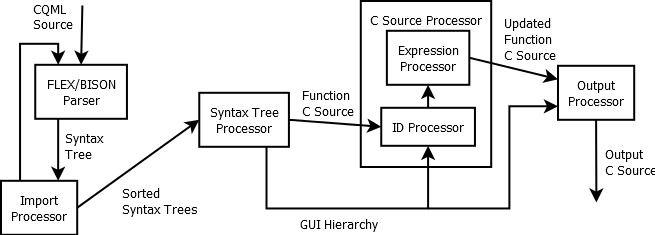
\includegraphics[width=0.7\textwidth]{parserdiag}
\caption{{\label{fig:fig1}}Návrh struktury překladače.}
\end{center}
\end{figure*}
Cílem prvního bloku (FLEX/BISON Parser) je přečíst zdrojový kód z CQML souboru a ověřit jeho syntaktickou správnost. V případě, že je kód syntakticky v pořádku, bude výstupem tohoto bloku syntaktický strom. Pro tento blok budou použity zdrojové kódy vygenerované pomocí aplikací Bison a Flex, z YACC gramatiky pro CQML.\\
V syntaktickém stromu budou nalezeny příkazy pro import souborů (blok Import Processor). Tyto soubory budou následně otevřeny a postupně zpracovány totožným způsobem.\\
Jakmile jsou všechny importované soubory zpracovány a jsou jejich zpracováním vytvořeny jejich syntaktické stromy, bude zjištěno, zda jsou některé soubory cyklicky závislé. To se bude realizovat pomocí konstrukce orientovaného grafu, kde každý vrchol představuje soubor a závislost mezi soubory je znázorněna hranou (směřující k importovanému souboru), a následným zjištěním zda v grafu existuje orientovaný cyklus. Pokud v grafu takový cyklus existuje, pak jsou soubory cyklicky závislé, což vyústí v chybu a ukončení programu. Je-li graf acyklický, jsou podle něho topologicky seřazeny syntaktické stromy jednotlivých souborů (vrcholy) pro následné zpracování.\\
V dalším bloku (Syntax Tree Processor) se zpracuje syntaktický strom a podle něj se vytvoří GUI hierarchie. Pro každý uzel představující GUI element, atribut, funkci, či nový atribut se vytvoří instance příslušné třídy. Každému elementu jsou podle jeho potomků v syntaktickém stromu přiřazeny jeho potomci v GUI hierarchii a jeho atributy a funkce.
Následně se zpracují všechny elementy s definovaným atributem ID, a tyto identifikátory se použijí ke tvorbě mapy, pomocí níž bude umožněno přistupovat k danému elementu podle definovaného identifikátoru.\\
V další části programu (C Source Processor) se zpracují kódy funkcí do formy potřebné pro závěrečný výstup v jazyce C. 

\subsection{Zpracování kódu v jazyce C}
Syntaktické stromy jednotlivých funkcí (případně výrazů) se projdou a převedou se na pole samostatných tokenů, takovým způsobem, že jeden prvek v poli bude představovat list stromu. Vzhledem k nutnosti kontroly existence atributů, budou pro snadnější zpracování některé tokeny v poli seskupeny do jednoho, který bude mít v sobě uloženo pole tokenů, které seskupil. Vzhledem k tomu, že každý token může obsahovat další tokeny, se bude stále jednat o stromovou strukturu, nicméně, bude mít nižší hloubku.\\
\begin{figure*}[!ht]
\begin{center}
  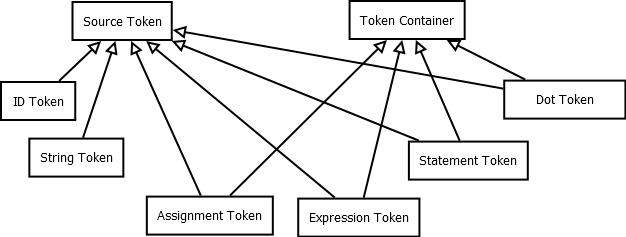
\includegraphics[width=0.7\textwidth]{tokens}
\caption{{\label{fig:fig2}}Diagram tříd tokenů.}
\end{center}
\end{figure*}

Na obrázku Figure \ref{fig:fig2} je znázorněn diagram tříd tokenů. Všechny tokeny dědí z jedné abstraktní třídy "Source Token". Vhledem k tomu, že pro implementaci překladače byl zvolen jazyk C++, je využito mnohonásobné dědičnosti a tokeny, jež sdružují skupinu tokenů do jednoho, dědí z třídy "Token Container". "ID Token" představuje nějaký identifikátor uvnitř kodu, zatímco "String Token" představuje jakýkoli jiný řetězec. "Dot Token" sdružuje tokeny pro výraz, v němž se pomocí operátoru "." přistupuje k atributům. "Statement Token" představuje libovolný výrok, "Assignment Token" představuje přiřazovací výraz a třída "Expression Token" libovolný jiný výraz.

\subsubsection{Zpracování identifikátorů}
Kódy (resp. syntaktické stromy) jednotlivých funkcí se projdou, a naleznou se identifikátory, jež se nachází v mapě identifikátorů elementů (id atributy elementů), a tyto identifikátory se v kódu nahradí skutečným názvem elementu uvnitř výsledné GUI aplikace.
\subsubsection{Dynamická kontrola typů a přiřazování hodnot}
Jelikož bude do atributů některých typů umožněno ukládat reference na objekty různého typu a pomocí této reference bude možné přistupovat k atributu daného objektu, nemůže být zaručeno, že atribut, ke kterému se aplikace snaží přistoupit, je v daném objektu přítomen. Proto bude potřeba za běhu výsledné GUI aplikace (využívající kód na výstupu překladače) kontrolovat přítomnost takového atributu.\\
Uvažujme kód z obrázku níže(viz.). Z kódu je zřejmé, že u atributu ref budepotřeba zkontrolovat, zda má objekt referovaný tímto atributem atribut ref2 a objekt referovaný ref2 obsahuje ref3.

\begin{lstlisting}[frame=single,caption=Pseudokód problematického použití operátoru "." v přiřazovacím výroku. ]
ref1 = ref1.ref2.ref3 = ref1.ref2.ref3
\end{lstlisting}
Oproti nahrazení identifikátoru názvem elementu nestačí pouze nahradit část textového řetězce ve výrazu. Vzhledem k tomu, že kromě ověření existence atributu bude potřeba daný atribut i získat pro další zpracování, bude nutné kód rozdělit do jednotlivých částí a každý operátor tečky nahradit voláním funkce pro získání (resp. nastavení) hodnoty atributu a kontrolou existence daného atributu.  Jak je znázorněno v kódu viz.
\begin{lstlisting}[frame=single,caption=Řešení v pseudokódu problematického použití operátoru "." v přiřazovacím výroku. ]
if(not CheckExistence(ref1, "ref2"))
	ReportException
var1 = ref1.Get("ref2");
if(not CheckExistence(var1, "ref3"))
	ReportException
var2 = var1.Get("ref3");

if(not CheckExistence(ref1, "ref2"))
	ReportException
var3 = ref1.Get("ref2");
if(not CheckExistence(var3, "ref3"))
	ReportException
var3.Set("ref3",var2);

Set("ref1",var2)
\end{lstlisting}
Díky možnosti zřetězit za sebou několik operátoru přiřazení, je potřeba rozdělit výraz na jednotlivé l-hodnoty a r-hodnoty a podle nich vybrat zda bude použit funkce pro získání nebo nastavení atributu, neboli l-hodnoty se nastaví tzv. setterem (tj. metoda pro nastavení atributu) a r-hodnoty se získají pomocí tzv. getteru (tj. metoda pro získání hodnoty atributu). Operátor "." pro přístup k atributu se zpravidla nahradí getterem, jedinou výjimku tvoří nejpravější operátor "." u nějaké l-hodnoty, neboli operátor "." nacházející se nejblíže nalevo od nějakého operátoru přiřazení.

\subsection{Výstup}
Poslední blok se postará o výpis do výstupních souborů. Pro každý zpracovaný vstupní soubor se vytvoří hlavičkový soubor s deklarací struktur a hlaviček funkcí. Každý soubor bude mít vlastní inicializační funkci pro inicializaci hierarchie a počátečnímu přiřazení hodnot a ukazatelů na potřebné funkce.\\
Pro každý GUI element, kterému je pomocí příkazu přidán nový atribut, se definuje nový typ struktury, která dědí z původního typu struktury. Každý přidaný atribut se deklaruje v nové struktuře, spolu s ukazatelem na funkci, která bude sloužit k jeho updatování. Pro každou takovou strukturu se také vytvoří funkce, které takovou strukturu alokují a inicializují, přičemž se v dané funkci zavolá funkce pro inicializaci struktury, ze které se dědí.\\
Pro všechny elementy se vytvoří funkce pro jejich update, která slouží k updatování hodnot v atributech elementů. Pro každý atribut, jemuž je přiřazena nějaká hodnota v CQML souborech, bude definována funkce pro jeho update danou hodnotou. Ukazatel na danou funkci, bude přiřazena v inicializační funkci daného souboru, do členské proměnné struktury určené pro daný atribut.\\



\section{\label{SEC:Intro}Implementace}

\subsection{Zpracování vstupu}
Pomocí generátoru Bison byl podle gramatiky jazyka CQML vytvořen parser. Pro vygenerování lexikálního analyzátoru byl použit FLEX. Zdrojový kód parseru a lexikálního analyzátoru je pak použit v překladači.
Po spuštění program načte výchozí typy GUI elementů, uloží si jejich názvy a seznam jejich atributů, včetně jejich typů a výchozích hodnot, do instancí třídy "ClassContainer".\\
Program na vstupu přijímá jméno souboru, se zdrojovým kódem v jazyce CQML. Pokud daný soubor existuje, je otevřen a jeho obsah je předán parseru. Pokud parser detekuje syntaktickou chybu ve zdrojovém souboru, vypíše chybu a program se ukončí. Výstupem parseru je syntaktický strom. V první fázi se ve stromu vyhledají příkazy pro import elementu z jiných souborů. Totéž program cyklicky provede pro všechny soubory, z nichž se elementy importují.

\subsection{Konstrukce a zpracování pomocných struktur}
Následně je vytvořen orientovaný graf vzájemných závislostí mezi jednotlivými soubory, kde každý vrchol představuje soubor a každá hrana představuje vazbu mezi soubory, zatímco počátečním vrcholem hrany je vrchol představující soubor, do něhož je element importován, a koncovým vrcholem je vrchol představující soubor, z nějž byl element importován. Pomocí algoritmu prohledávání do hloubky je zjištěno, zda se v grafu nachází cyklus. Pokud se v grafu nachází cyklus, je vypsána chybová hláška a program se ukončí.\\
Jelikož je graf acyklický, pak každý vrchol představuje komponentu a tak lze jednotlivé vrcholy grafu a tudíž i soubory topologicky seřadit. Soubory (resp. vrcholy v grafu) jsou seřazeny pomocí Tarjanova algoritmu. Syntaktické stromy jednotlivých seřazených souborů jsou postupně zpracovány následujícím způsobem.\\
Během průchodu stromem se postupně alokují instance třídy Element, přičemž každá instance představuje určitý element v hierarchii GUI. Každému elementu je přiřazen jeho typ a seznam jeho potomků resp. elementů, které se v hierarchii nachází níže. Dále je každému elementu, u nějž jsou definované změny některých z jejich atributů, přiřazena množina dvojic názvů atributů a jejich hodnot. Hodnotou v tomto případě nemusí být konstanta, ale i výraz v jazyce C, jehož výpočtem se získá daná hodnota ve vygenerovaném zdrojovém kódu. Atributu může být také přiřazen kód celé funkce nejen samostatný výraz, v tomto případě by daná funkce vracela hodnotu atributu. Kód v jazyce C je ve formě syntaktického stromu předán funkci "SourceToHandler" (jedná-li se o celou funkci) nebo "ExpressionToHandler" (jedná-li se pouze o výraz). Výstupem obou funkcí je instance třídy "SourceHandler", která zdrojový kód v podobě posloupnosti tokenů, způsobem popsaným v kapitole (viz.). V tomto případě není tokenem myšlen pouze symbol či řetězec v syntaktickém stromu, jenž je výstupem parseru, ale i struktura obsahující pomocná data (např. informace o tom zda bude token nahrazen něčím jiným).\\
Dále program vytvoří mapu identifikátorů, pro všechny elementy, u nichž byl nastaven atribut "id". Tento atribut musí mít unikátní hodnotu, pokud je v souboru více než jeden element nastaven na stejnou hodnotu atributu "id", dojde k chybě. Pro každý soubor se uchovává jedna mapa identifikátorů.\\
Každému elementu je podle jeho specifikovaného typu přiřazen ukazatel na instanci "ClassContainer". Pokud byly nějakému elementu přiřazeny nové atributy (pomocí klíčového slova property), bude muset být ve výstupním kódu daný element reprezentován speciální třídou, tudíž se vytvoří nová instance "ClassContainer", do které jsou mimo výchozích atributů přidány i atributy nové. Všechny nové atributy musí být buď nějakého výchozího typu, nebo musí typem nějakého importovaného či výchozího elementu, jinak dojde k chybě.

\subsection{Zpracování kódu v jazyce C}
Vzhledem k tomu, že se lze v částech, které jsou napsané v jazyce C, odkazovat na jiné elementy pomocí jejich identifikátorů "id", je nutné analyzovat výrazy a nahradit ve výsledném kódu identifikátory referencemi na dané elementy. To je vyřešeno projitím všech tokenů, jež obsahují identifikátor, a vyhledáním příslušného identifikátoru v mapě identifikátorů (pro právě zpracovávaný soubor). Je-li identifikátor nalezen, pak se k příslušnému tokenu zapíše, že má být ve výstupu nahrazen referencí na identifikovaný element.\\
Následně se v kódu zpracují všechny operátory "." pro přístup k atributu tak, že se každý takový operátor nahradí voláním funkce pro nastavení nebo získání hodnoty atributu. V případě, že se operátor "." nachází nejblíže nalevo od operátoru přiřazení, nahradí se funkcí pro nastavení (setterm), v opačném případě funkcí pro získání hodnoty (getterem), jako je tomu (viz.). Pro ukládání výsledků těchto funkcí se používají pomocné proměnné. Vzhledem k tomu, že se mohou tyto operátory nacházet uvnitř výrazů, je celý řetězec operátorů "." nahrazen až názvem proměnné, ve které je uložen výsledek posledního z nich a volání funkcí, jež jejich funkčnost nahrazuje, se připojí před začátek výroku, ve kterém se nachází. Začátek výroku je symbolizován specifickým tokenem, a tudíž se volání funkcí připojí k němu v podobě datové struktury udávající typ funkce a jména pomocných proměnných, což bude použito při generování výstupu.


\subsection{Výstup}
Na závěr jsou pro každý zpracovaný soubor vytvořeny tři výstupní soubory, jejichž názvy jsou zakončeny ".h", ".c", "outer.h". 
Do prvního souboru ("*.h") jsou zapsány hlavičky konstruktorů hlavní komponenty a také definice této komponenty, respektive struktury, jenž ji reprezentuje, tudíž se do těla struktury vypíší členské proměnné (reprezentujících GUI elementy v komponeně). Pro každý nový typ definovaný ve zpracovávaném souboru (reprezentovaný instancí třídy "ClassContainer") se vytvoří totéž, přičemž do těla struktury se jako členské proměnné vypíší atributy třídy, avšak první členskou proměnnou bude proměnná typu struktury, jenž představuje element, z něhož tento nový element vychází (tímto se realizuje dědičnost v jazyce C).\\
Do druhého souboru ("*.c") jsou zapsány definice všech vygenerovaných funkcí. Každý atribut má také přidělenou funkci, která se stará o jeho update. Struktura obsahující atribut obsahuje i ukazatel na danou funkci. Do těla takové funkce je zapsán kód výrazu nebo funkce, přiřazený danému atributu v CQML souboru, který byl upraven a nyní je uložen v instanci třídy "SourceHandler" příslušící danému atributu.\\
Každá struktura má definovány dva konstruktory, jeden inicializuje instanci struktury, přiřadí každému atributu počáteční hodnotu a všem ukazatelům na funkce příslušnou funkci, a druhý alokuje paměť pro danou strukturu a poté zavolá první konstruktor. Jelikož jazyk C nepodporuje konstruktory struktur, je zde pojmem konstruktor myšlena funkce pro vytvoření instance struktury.\\
Do třetího souboru ("*outer.h") jsou jsou zapsány pouze hlavička konstruktoru hlavní komponenty souboru a deklarace struktury představující hlavní komponentu. Tento soubor slouží k začlenění do souboru, jež danou komponentu bude používat.\\
Jakmile jsou takto zpracovány všechny vstupní soubory, vytvoří se poslední výstupní soubor, ve kterém se definuje hlavní inicializační funkce, ve které se vytvoří instance hlavní komponenty GUI (komponenta prvního souboru, který byl programu zadán), a také funkce pro volající update této komponenty.\\


\section{\label{SEC:Conclusion}Závěr}
Výstupem této práce je jazyk CQML pro deklarativní definici GUI, který se svou syntaxí velice blíží jazyku QML. Dalším výstupem je překladač, který přeloží kód z jazyka CQML do jazyka C++, který by měl jít integrovat do aplikace, která by poskytovala potřebný backend zajišťující vstup, výstup a run-time správu GUI. Potřebný backend bohužel nebyl během této práce dokončen.\\
Na toto téma by bylo možné navázat další prací, která by se zabývala rozšířením funkčnosti jazyka a překladače CQML a také implementací knihovny poskytující potřebný backend pro fungování GUI v aplikaci, do které by se mělo integrovat.

\clearpage
\section{\label{SEC:APA}Příloha A - Gramatika }
Následuje soubor pravidel pro gramatiku ve formátu YACC pro jazyk CQML. Terminály jsou psané velkým písmem a neterminální symboly malým. Neterminály "compound\_statement", "type\_specifier" a "conditiona\_lexpression" jsou převzaty z gramatiky pro jazyk C, a jejich zpracování bude provedeno podle pravidel gramatiky jazyka C.
\begin{lstlisting}[frame=single,caption=Gramatika jazyka CQML,label=lst:g]
start_point
	:	element_or_import_list
;

element_or_import_list
	:	import_list element
	|	element
;

import_list
	:	import import_list
	|	import
;

import
	:	IMPORT STRING_LITERAL AS IDENTIFIER
;
element
	:	IDENTIFIER '{' attribute_or_subelement_list '}'
	|	IDENTIFIER '{' '}'
;
attribute_or_subelement_list
	: attribute_or_element ';' attribute_or_subelement_list
	| attribute_or_element ';'
;


attribute_or_element
	: element
	| event_handler
	| attribute
	| property
;


event_handler
	: IDENTIFIER ':' compound_statement
;

property
	: PROPERTY IDENTIFIER attribute
	| PROPERTY type_specifier attribute
	| PROPERTY IDENTIFIER IDENTIFIER
	| PROPERTY type_specifier IDENTIFIER
;


attribute
	:	IDENTIFIER ':' conditional_expression
	|	IDENTIFIER '.' IDENTIFIER ':' conditional_expression
;
\end{lstlisting}

\clearpage
\section{\label{SEC:APB}Příloha B - Použité technologie }

\subsubsection{Flex}
Flex je nástroj pro tvorbu skenerů pro lexikální analýzu. Jeho cílem je rozpoznat lexikální šablony v textovém vstupu a převést je na výstup ve formě posloupnosti symbolů (tokenů), které mohou být zpracovány dále například pomocí parseru.
\subsubsection{Bison}
Bison je víceúčelový generátor parserů, který z dané bezkontextové gramatiky vygeneruje deterministický LR parser nebo generalizovaný LR parser ve formě zdrojového kódu k programu v jazyce C nebo C++.


\end{document}
